\renewcommand\thesection{VII}
\section{Courant Électrique, Résistance, Piles}
\begin{multicols*}{2}
    \subsection{Courant Électrique}
    
    L'intensité $I$ du courant électrique est une mesure de la charge traversant une surface par unité de temps.
    \[ I = \frac{dQ}{dt} \]
    
    Avec $I$ en Ampères ($A$):
    \[ 1 A = \frac{1 C}{s} \]
    
    \paragraph{Direction de mouvement du courant et des électrons}
    
    \begin{center}
        \begin{circuitikz}
            \draw (0, 0) to [battery1, i=$I$] (3, 0) to (3, 2) to node[above, pos=0.5] {$\leftarrow e^-$} (0,2) to (0,0);
        \end{circuitikz}
    \end{center}
    
    Les électrons vont de la borne négative à la borne positive, alors que le courant va dans le sens inverse: de la borne positive vers la borne négative de la pile.
    
    \subsection{Résistance et Loi d'Ohm}
    \[ R = \frac{V}{I} \]
    
    R est une réststance en Ohm ($\Omega$). Une résistance d'1$\Omega$ laisse passe un courant d'1$A$ lorsqu'on lui applique un tension d'1$V$.
    
    \[ 1 \Omega = \frac{1V}{A} \]
    
    \paragraph{Loi d'Ohm}
    Pour un conducteur Ohmique avec $R$ constant:
    \[ V = RI \]
    
    \subsubsection{Résistances Ohmiques}
    
    \begin{center}
        \begin{circuitikz}
            \draw (0, 0) to [R = $R$] (3, 0);
        \end{circuitikz}
    \end{center}
    
    \paragraph{Conducteur Ohmique}
    Conducteur dont la fonction $I = f(V)$ est linéaire.
    
    \begin{center}
        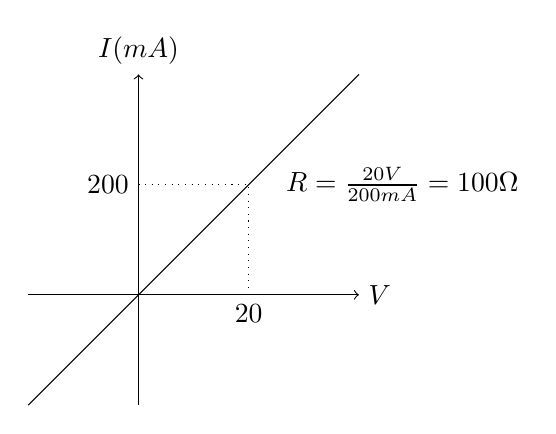
\begin{tikzpicture}[scale=0.7]
            \draw[->] (0, -2) -- (0, 4) node[above] {$I(mA)$};
            \draw[->] (-2, 0) -- (4, 0) node[right] {$V$};
            \draw (-2, -2) -- (4, 4);
            \draw[dotted] (0, 2) node[left] {$200$} -- (2, 2) node[right] {$\quad R = \frac{20V}{200mA} = 100 \Omega$} -- (2, 0) node[below] {20};
        \end{tikzpicture}
    \end{center}
    
    \subsubsection{Résistances non Ohmique}
    
    
    \begin{center}
        \begin{circuitikz}
            \draw (0, 0) to [diode] (3, 0);
        \end{circuitikz}
    \end{center}
    \paragraph{Diode} Élément qui n'obéit pas à la loi d'Ohm et qui ne laisse passer le courant que dans un sens.
    
    \begin{center}
        \begin{tikzpicture}[scale=0.7]
            \draw[->] (0, -3) -- (0, 3) node[above] {$I$};
            \draw[->] (-3, 0) -- (3, 0) node[right] {$V$};
            \draw (-2, -3) -- (-2, -0.25) .. controls (0,-0.06) .. (0.7, 0.25) .. controls (0.8, 0.5) .. (1, 3);
            \draw (0.7, 0) node[below] {\footnotesize 0.7} -- (0.7, 0.1);
            \draw (-2, 0) node[above] {\footnotesize -100} -- (-2, 0.1);
            \draw (0,1) node[left] {\footnotesize $10 mA$} -- (0.1, 1);
            \draw (0,-1) node[left] {\footnotesize $-1\mu A$} -- (0.1, -1);
        \end{tikzpicture}
    \end{center}
    
    \subsection{Résistivité et Conductivité}
    
    \paragraph{Résistance d'un fil homogène}
    La résistance d'un fil de longueur L et d'aire de section A est donnée par
    \[ R = \rho \frac{L}{A} \]
    
    Où $\rho$ est une constante de proportionnalité: la résistivité.
    
    \subsubsection{Résistivité}
    
    La résistivité d'un matériau est exprimée en Ohm-mètres ($\Omega m$).
    
    Pour les métaux, elle augmente linéairement avec la température: plus d'agitation dans le matériau empêche les électrons de passer.
    
    \[ \rho_t = \rho_0 (1 + \alpha (T-T_0)) \]
    
    Avec $\rho_0$ la résistivité à une température de référence $T_0$, et $\alpha$ le coéfficient thermique de résistivité ($\frac{1}{°C}$).
    
    \subsubsection{Conductivité}
    
    Tout simplement l'inverse de la résistivité $\rho$
    \[ \sigma = \frac{1}{\rho} \]
    
    \subsection{Force Électro-Motrice et Tension aux Bornes}
    
    Une source de force électro-motrice (ou f.é.m.) est un instrument qui transforme un type d'énergie (chimique, cinétique, ...) en énergie électrique.
    \paragraph{Exemples} Pile, Générateur, ...
    
    \paragraph{Force Électro-Motrice} Différence de potentiel aux bornes de $\xi$
    
    \begin{center}
        \begin{circuitikz}
            \draw (0, 0) node[above] {$a$} [R = $r$, *-] to (3, 0) to [battery1, l^=$\xi$, -*] (5, 0) node[above] {$b$};
        \end{circuitikz}
    \end{center}
    
    Une source de f.é.m contient souvent une résistance interne $r$. Celle-ci est due au frein des électrons au sein de la source de f.é.m. Ceci implique que la différence de potentiel mesurée à ses bornes est différente de la f.é.m. nominale:
    \[ V_{ab} = \xi - rI \]
    
    \subsection{Puissance Électrique}
    
    En parcourant les fils, les électrons de conduction percutent les atomes du matériau les composant. L'énergie cinétique des atomes augmente, ce qui fait monter la température.
    
    \paragraph{Puissance d'un appareil électrique}
    
    \[P = \frac{dU}{dt} = \frac{dq}{dt}V \]
    \[\Leftrightarrow P = IV = RI^2 = \frac{V^2}{R} \]
    
    \subsection{Courant Alternatif}
    
    \paragraph{Courant Continu -- DC} (Direct Current), l'intensité du courant reste constant dans le temps.
    \begin{center}
        \begin{tikzpicture}[scale=0.5, smooth]
            \draw[->] (0, -1) -- (0, 4) node[above] {I(t)};
            \draw[->] (-1, 0) -- (10, 0) node[right] {t};
            \draw (0, 3) node[left] {$I_0$} -- (10, 3) node[above] {$I(t) = I_0$};
        \end{tikzpicture}
    \end{center}
    
    \paragraph{Courant Alternatif -- AC} (Alternative Current), l'intensité du courant varie avec le temps. Usuellement de forme sinusoïdale.
    \begin{center}
        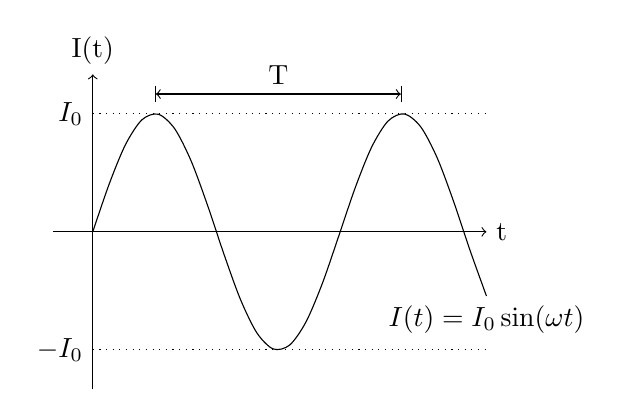
\begin{tikzpicture}[scale=0.5, domain=0:10, smooth]
            \draw[->] (0, -4) -- (0, 4) node[above] {I(t)};
            \draw[->] (-1, 0) -- (10, 0) node[right] {t};
            \draw plot (\x, {3 * sin(\x r)}) node[below] {$I(t) = I_0 \sin(\omega t)$};
            \draw[dotted] (0, 3) node[left] {$I_0$} -- (10, 3);
            \draw[dotted] (0, -3) node[left] {$-I_0$} -- (10, -3);
            \draw[|<->|] ({pi/2}, 3.5) -- ({5* pi/2}, 3.5) node[above, pos=0.5] {T};
        \end{tikzpicture}
    \end{center}
    
    Avec $\omega = 2\pi f$ avec la fréquence du courant des centrales Belges $f=50Hz$.
    
    \subsubsection{Courant Fourni par une Génératrice}
        \[ I = I_0 \sin(\omega t) \]
        \[ V = RI = RI_0\sin(\omega t) = V_0 \sin(\omega t) \]
    Avec la tension maximale $V_0 = RI_0$
    
    \subsubsection{Puissance Instantanée}
    \[ P(t) = RI^2(t) = RI_0^2\sin^2(\omega t) \]
    
    \subsubsection{Puissance Moyenne}
    \[ P_m = \frac{1}{2} I_0^2 R \]
    
    La puissance moyenne d'un courant AC d'amplitude $I_0$ dans une résistance R est égale à la puissance dissipée par un courant continu:
    \[ I_{\text{eff}} = \frac{I_0}{\sqrt{2}} \quad \text{avec} \quad V_{\text{eff}} = \frac{V_0}{\sqrt{2}} \]
    
    \[ P_m = V_{\text{eff}} I_{\text{eff}} = \frac{V_{\text{eff}}^2}{R} = RI_{\text{eff}}^2 \]
    
    
\end{multicols*}
